\documentclass{paper}

%\usepackage{times}
\usepackage{epsfig}
\usepackage{graphicx}
\graphicspath{{superresolution/}{superresolution/output/}}
\usepackage{amsmath}
\usepackage{amssymb}
\usepackage{color}
\usepackage{hyperref}
\usepackage[tight,footnotesize]{subfigure}

% load package with ``framed'' and ``numbered'' option.
%\usepackage[framed,numbered,autolinebreaks,useliterate]{mcode}

% something NOT relevant to the usage of the package.
\setlength{\parindent}{0pt}	
\setlength{\parskip}{18pt}
\newcommand{\norm}[1]{\left\lVert#1\right\rVert}

\usepackage[latin1]{inputenc} 
\usepackage[T1]{fontenc} 

\usepackage{listings} 
\lstset{% 
   language=Matlab, 
   basicstyle=\small\ttfamily, 
} 

\title{Assignment 1}



\author{Moser Stefan\\09-277-013}
% //////////////////////////////////////////////////


\begin{document}



\maketitle


% Add figures:
%\begin{figure}[t]
%%\begin{center}
%\quad\quad   \includegraphics[width=1\linewidth]{ass2}
%%\end{center}
%
%\label{fig:performance}
%\end{figure}

\section*{Superresolution}

\subsection*{Problem}
Through various effects, an image may end up with a low resolution. 
This can be due to hardware limitations 
(e. g. an image taken from a cheap security camera), 
bandwith limitations 
(e. g. an image was downscaled for transmitting over a connection with very low bandwith) or others.  


\subsection*{Motivation}
To retrieve further details, we might now want to increase image quality by increasing its resolution. 
While this is not possible in a manner as depicted in \href{http://petapixel.com/2012/08/17/ridiculous-photo-enhancement-scene-from-the-tv-show-csi/}{popular TV series}, 
we can make certain assumptions for regularization combined with convex optimization to increase quality by a fair amount. 
In this project use a regularization term that penalizes high gradients,
assuming that the original image largely consists of smooth patches.

\subsection*{Derivation of Gradient}

The energy term we want to optimize in this problem is 
\begin{equation}
E(u) = \norm{\nabla u} + \frac{\lambda}{2} \norm{Du - g}^2_2.
\end{equation}
The left summand we will further call regularisation term, 
the right one fitting term. 

The regularisation term consists only of the gradient
of the superresolution image $u$, conserving the smoothness of the image.
While any norm would be acceptable, I chose the 2-norm for its nice
mathematical properties.

The fitting term consists of the channel selector $D$, 
the superresolution image $u$ and the initial image $g$ (with low resultion).
This term ensures that the optimum
\begin{equation}
\tilde{u} = \min_{u \in X} E(u) = \min_{u \in X} \norm{\nabla u} + \frac{\lambda}{2} \norm{Du - g}^2_2
\end{equation}
stays close to the initial
image when applying the channel selector. 

The fitting term on the right can be derived pretty easily using the chain rule
\begin{align}
\frac{\partial E(u)}{\partial u} 
&= \norm{\nabla u} + \frac{\lambda}{2} (Du - g)^T(Du - g) \frac{\partial}{\partial u} \\
&= \norm{\nabla u} \frac{\partial}{\partial u} + D^T D u - D^T g
\end{align}
by expressing the images $u$ and $g$ as vectors. For further use, we define
this term as 
\begin{equation}
 f = D^T D u - D^T g
\end{equation}
The regularization term however needs some more work. 
For this purpose we first discretize the norm of the gradient as
\begin{equation}
\norm{\nabla u} \approx \sum_{i,j} 
	\sqrt{(u[i+1,j] - u[i,j])^2 + (u[i, j+1] - u[i, j])^2}
\end{equation}
One single term of this sum can then be expressed as
\begin{equation}
\tau[i,j] = \sqrt{(u[i+1,j] - u[i,j])^2 + (u[i, j+1] - u[i, j])^2}
\end{equation}
Using these tools, we can now easily define the gradient of the regularization term in a single component as
\begin{equation}
\frac{\partial \norm{\nabla u}}{\partial u[i,j]} = 
	\frac{\partial \tau[i,j]}{\partial u[i,j]} +
	\frac{\partial \tau[i - 1,j]}{\partial u[i,j]} +
	\frac{\partial \tau[i,j - 1]}{\partial u[i,j]}
\end{equation}
With all other terms being independent of $u[i,j]$ and thus being zero.
These three expressions can now be computed as
\begin{align}
\frac{\partial \tau[i,j]}{\partial u[i,j]} 
&= &&\frac{\partial \sqrt{(u[i+1,j] - u[i,j])^2 + (u[i, j+1] - u[i, j])^2}}{\partial u[i,j]} \\
&= &&\frac{1}{2} ((u[i+1,j] - u[i,j])^2 + (u[i, j+1] - u[i, j])^2)^{-\frac{1}{2}} \\
& &&\frac{\partial}{\partial u[i,j]} 
(u[i+1,j] - u[i,j])^2 + (u[i, j+1] - u[i, j])^2 \\
&= &&\frac{1}{2}\tau[i,j]^{-1} \\
& &&\frac{\partial}{\partial u[i,j]} 
(u[i+1,j] - u[i,j])^2 + (u[i, j+1] - u[i, j])^2 \\
&= &&\frac{1}{2}\tau[i,j]^{-1}
(-2(u[i + 1, j] - u[i,j]) - 2(u[i, j+1] - u[i,j])) \\
&= &&\tau[i,j]^{-1} (2 u[i,j] -u[i + 1, j] - u[i, j+1]) \\
&= &&\frac{2u[i,j] - u[i + 1, j] - u[i, j+1]}{\tau[i,j]}
\end{align}
In a similar fashion, we can compute the partial derivatives for
$\tau[i-1, j]$ and $\tau[i, j - 1]$
\begin{align}
\frac{\partial \tau[i - 1,j]}{\partial u[i,j]} 
&= &&\frac{\partial \sqrt{(u[i,j] - u[i-1,j])^2 + (u[i-1, j+1] - u[i-1, j])^2}}{\partial u[i,j]} \\
&= &&\frac{1}{2} \cdot \frac{1}{\tau[i - 1, j]} \cdot 2 \cdot (u[i,j] - u[i-1, j]) \\
&= &&\frac{u[i,j] - u[i-1, j]}{\tau[i - 1, j]}
\end{align}
respectively
\begin{align}
\frac{\partial \tau[i,j-1]}{\partial u[i,j]} 
&= &&\frac{\partial \sqrt{(u[i + 1 ,j] - u[i,j - 1])^2 + (u[i, j] - u[i, j - 1])^2}}{\partial u[i,j]} \\
&= &&\frac{1}{2} \cdot \frac{1}{\tau[i, j - 1]} \cdot 2 \cdot (u[i,j] - u[i, j-1]) \\
&= &&\frac{u[i,j] - u[i, j - 1]}{\tau[i, j-1]}
\end{align}

The $\tau$ terms need additional care, since they appear in the denominator
of the fractions. To prevent division by zero and increase numerical 
stability, we add we approximate them as 
\begin{equation}
\tilde{\tau}[i,j] = \sqrt{(u[i+1,j] - u[i,j])^2 + (u[i, j+1] - u[i, j])^2 + \delta}
\end{equation}
with $\delta$ being a small positive number.

Combining our efforts from before, we can express the gradient of the objective function as
\begin{align}
\nabla E[i] = &\frac{u[i,j] - u[i-1, j]}{\tilde{\tau}[i - 1, j]} + \\
	&\frac{u[i,j] - u[i, j - 1]}{\tilde{\tau}[i, j-1]} + \\
	&\frac{u[i,j] - u[i, j - 1]}{\tilde{\tau}[i, j-1]} + \\
	&f[i]
\end{align}

\subsection*{Implementation}

\subsubsection*{Iteration count}
In my implementation, I used $Dg$ as initial guess. While around 5000 iterations
seemed to be enough in most cases, I went up to 10'000 iterations to be sure there
is no misleading effect due to low iteration count.

\begin{figure}[ht!]%
\centering
\subfigure[0 Iterations]{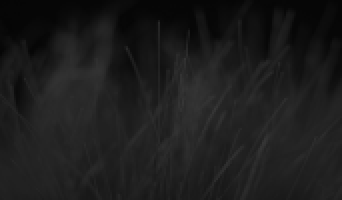
\includegraphics[width=0.32\textwidth]{grass_small_lambda_700_iteration_0.png}}
\subfigure[1000 Iterations]{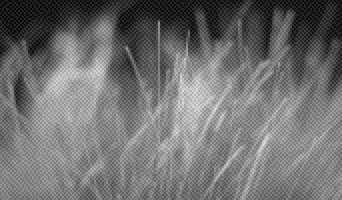
\includegraphics[width=0.32\textwidth]{grass_small_lambda_700_iteration_1000.png}}
\subfigure[2000 Iterations]{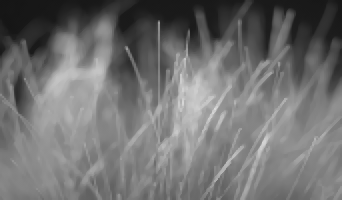
\includegraphics[width=0.32\textwidth]{grass_small_lambda_700_iteration_2000.png}} \\
\subfigure[4000 Iterations]{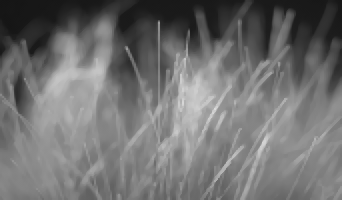
\includegraphics[width=0.32\textwidth]{grass_small_lambda_700_iteration_4000.png}} 
\subfigure[6000 Iterations]{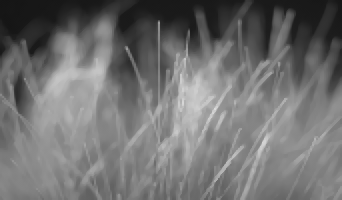
\includegraphics[width=0.32\textwidth]{grass_small_lambda_700_iteration_6000.png}} 
\subfigure[8000 Iterations]{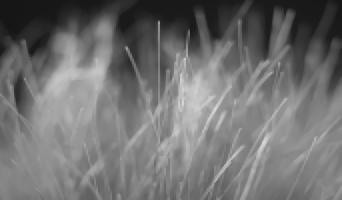
\includegraphics[width=0.32\textwidth]{grass_small_lambda_700_iteration_8000.png}} 
\caption{The superresolution image after various iteration counts.
Iteration 0 shows the initial guess. After iteration 4000 there are only
minor changes. The lambda was set to 700 for these images.}
\label{fig:iteration_count}
\end{figure}

\subsubsection*{Effect of Lambda}
As can be seen in Figure \ref{fig:lambdas}, the lambda defines the smoothness
of the resulting image. 
Surprisingly, 
the quality only deteriorates with extremely large lambdas. 
The choose of lambda also impacts the choose of the learning rate: 
With a large lambda, the learning rate has to be lowered in order for the
optimization to not become unstable.
\begin{figure}[ht!]%
\centering
\subfigure[$\lambda = 10$]{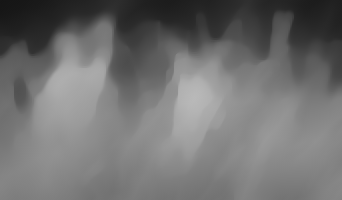
\includegraphics[width=0.32\textwidth]{grass_small_lambda_10_iteration_8000.png}}
\subfigure[$\lambda = 100$]{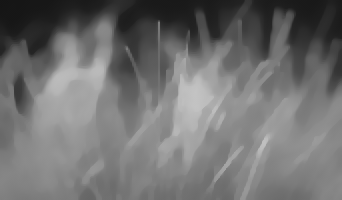
\includegraphics[width=0.32\textwidth]{grass_small_lambda_50_iteration_8000.png}}
\subfigure[$\lambda = 200$]{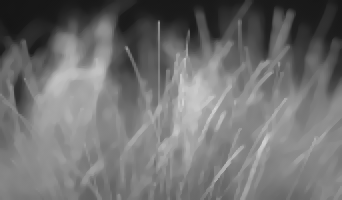
\includegraphics[width=0.32\textwidth]{grass_small_lambda_200_iteration_8000.png}} \\
\subfigure[$\lambda = 500$]{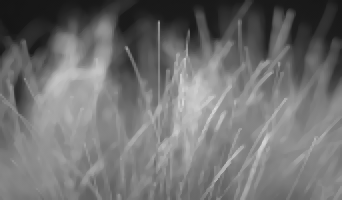
\includegraphics[width=0.32\textwidth]{grass_small_lambda_500_iteration_8000.png}} 
\subfigure[$\lambda = 700$]{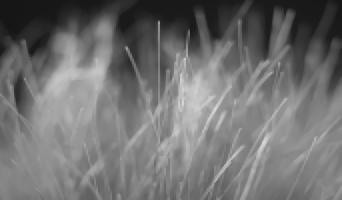
\includegraphics[width=0.32\textwidth]{grass_small_lambda_700_iteration_8000.png}} 
\subfigure[$\lambda = 1000$]{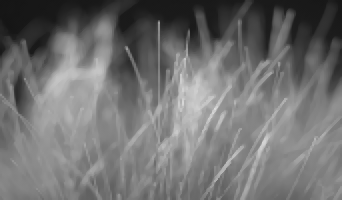
\includegraphics[width=0.32\textwidth]{grass_small_lambda_1000_iteration_8000.png}} 
\caption{Various resulting images with different lambdas after 8000 iterations.}
\label{fig:lambdas}
\end{figure}

\subsubsection*{Optimal Lambda}
\begin{figure}[ht!]%
\centering
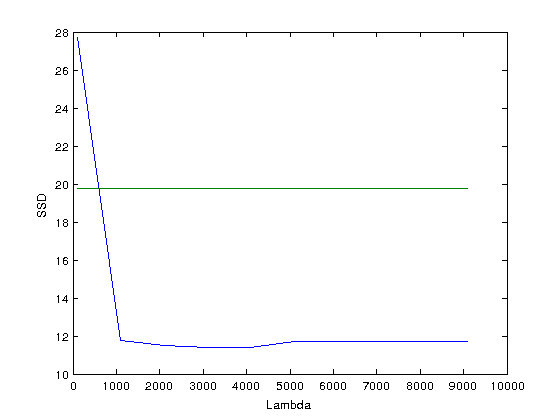
\includegraphics[width=0.9\textwidth]{lambda_vs_ssd.png}
\caption{Various resulting images with different lambdas after 8000 iterations.}
\label{fig:lambda_vs_ssd}
\end{figure}
I tested a wide variety of lambdas before concluding that the optimal lambda
is somewhere around 4000 (see Figure \ref{fig:lambda_vs_ssd}). The improvements above a lambda
of 1000 are marginal however. As already stated above, the results don't become
much worse when choosing even larger lambdas.

\end{document}
 
 